\subsection{Introduction and Related Work}
\label{subsubsec:furthers-cost-backgroung}
Through observation in following example, the heap resource consumption during the program 
execution is accumulating in the same way as the program's adaptivity. Specifically, in line 5 
where the list is re-written and the heap consumption is decreased implicitly. 
This implicit decrease 
of the cost works exactly the same as program's adaptivity decrease.
\\
This motivates the generalization of the analysis framework onto the program's resource cost analysis. Use this framework,
I will give
a more accurate resource cost estimation by taking the program's implicit resource cost into consideration, comparing 
to the worst case cost analysis in traditional way.
\\
There are two categories of the program cost analysis, Type-System Based and Static Program Analysis Based. But both of the
works in these two areas fails to recognize the case where program resource consumption is decreased implicitly.
\paragraph*{Type-System Based}
Existing
static program analysis based type-system are mainly through 
effect systems, 
% control-flow analysis, and data-flow analysis~\cite{ryder1988incremental}. 
% The idea of statically estimating a sound upper bound for the adaptivity from the semantics is indirectly inspired from prior work on cost analysis via effect systems~\cite{cciccek2017relational,radivcek2017monadic,qu2019relational}. The idea of defining adaptivity using data flow is inspired by the work of graded 
Hoare logic~\cite{gaboardi2021graded}, and amortized type system~\cite{hoffmann_jost_2022}.
%
In these system, the cost are accumulating through the type induction. The only way to save the cost into the potential
type, as in~\cite{GustafssonEL05} and \cite{hoffmann_jost_2022}, is through explicit abstraction or data structure de-allocation.
That is to say, they cannot deal with the case where the cost (for example the adaptivity) decreases when there isn't a dependency relation between variables.
\paragraph*{Static Program Analysis}
Existing static program analysis works via the control flow or data flow analysis 
in program resource cost analysis 
mainly falls into two areas, the program complexity analysis and worst case execution time analysis. 
They are focusing on analyzing the cost of the entire program. 
The techniques are based on
type system~\cite{CicekBG0H17, RajaniG0021}, Hoare logic~\cite{CarbonneauxHS15}, abstract interpretation~\cite{GustafssonEL05, HumenbergerJK18},
invariant generation through cost equations or ranking functions~\cite{BrockschmidtEFFG16,AlbertAGP08,AliasDFG10,Flores-MontoyaH14}
or a combination of program abstraction and invariant inferring~\cite{GulwaniZ10, SinnZV17,GulwaniJK09}.
In general, these techniques give the approximated upper bound of the program's total running time or resource cost.
However, they failed to consider the case where the cost -- the adaptivity-- could decrease when there isn't a dependency relation between variables.

\subsection{Motivating Example}
\label{subsubsec:furthers-cost-example}

\begin{example}
Now, I show an example illustrating how our two updating operations for adaptivity 
for each path can guarantee both the accuracy and the soundness. 
Look at a Nested While Loop example program in Figure~\ref{fig:alg_adaptsearch_nestedwhile}.
% Notice here, another special operation I have in the second branch is Non-updating of
% % Non-updating the 
% $\kw{querynum}$ and $\kw{flowcapacity}$.
% This guarantees both the accuracy and the soundness.
% Specifically,
% % because a second visiting of the same vertex 
% if this vertex is visited, it indicates that a cycle is monitored and  
% % indicates there is a cycle goes back to this vertex, 
% the traversing on this cycle is finished by going back to this vertex.
% %
% % then, when 
% When I continuously search for walks heading out of this vertex, 
% the minimum weight on this cycle does not affect the walks going out of this vertex that not pass this cycle.
% However, if I keep recording the minimum weight, then we
% %  are restricting 
% restrict the visiting times of vertices on a walk by
%  using the minimum weight of vertices not on this walk.
% %  , it is unsound anymore.
% Then, it is obviously that this leads to unsoundness.
% \todo{example} 
% To under stand how the two operations 
I first search for a path: $y^6 \to y^6$, and compute the adaptivity for this path as 
$k$.
Notice here, another special operation I have in the second branch is Non-updating of
% Non-updating the 
$\kw{querynum}$ and $\kw{flowcapacity}$.
This guarantees both the accuracy and the soundness.
Specifically,
% because a second visiting of the same vertex 
if this vertex is visited, it indicates that a cycle is monitored and  
% indicates there is a cycle goes back to this vertex, 
the traversing on this cycle is finished by going back to this vertex.
%
% then, when 
When I continuously search for walks heading out of this vertex, 
the minimum weight on this cycle does not affect the walks going out of this vertex that not pass this cycle.
However, if I keep recording the minimum weight, then we
%  are restricting 
restrict the visiting times of vertices on a walk by
using the minimum weight of vertices not on this walk.
%  , it is unsound anymore.
Then, it is obviously that this leads to unsoundness.
If I update the $\kw{flowcapacity}[y^6]$ as $k$ after visiting $y^6$ the second time 
on this walk,
% the walk $y^6 \to y^6$,
and continuously visit $x^9$,
then the $\kw{flowcapacity[k]}$ is 
updated as $\min(k, k^2)$.
So
%  which 
% restricting 
the visiting times of $x^9$ is restricted by $k$ on the walk $y^6 \to y^6 \to x^9$.
This restriction excludes the finite walk $y^6 \to y^6 \to x^9 \to x^9$ where $y^6$ and $x^9$ visited by $k^2$ times
in the computation. 
However, the finite walk $y^6 \to y^6 \to x^9 \to x^9$ where $y^6$ is visited $k$ times and $x^9$ $k^2$ times is 
a qualified walk, and exactly the longest walk I aim to find. So, by Non-updating the $\kw{flowcapacity}$ after 
visiting $y$ again, I guarantee that the visiting times og vertices on every searched walk will not be restricted by weights not on this walk,
i.e., the soundness.
\\
In the last line of this dfs algorithm, line: 16, it returns the adaptivity heading out from its input vertex.
\\
By applying this deep first search strategy on every vertex on this SCC, 
I compute the adaptivity of this SCC by taking the maximum 
% adaptivity reaching every vertex on this SCC.
value over every vertex.
%
The largest heap resource consmuption in total, by $y$ and $x$ together computed from the $\THESYSTEM$ is $1 + k^2 + k$.
Comparing to $k + k^2 + k^3$ estimated as  the longest weight path from traditional CFL-reachability method, 
my analysis improved the accuracy by $O(n)$.

% Look at a Nested While Loop example program in Figure~\ref{fig:alg_adaptsearch_nestedwhile}.
% Specifically,
% % because a second visiting of the same vertex 
% if this vertex is visited, it indicates that a cycle is monitored and  
% % indicates there is a cycle goes back to this vertex, 
% the traversing on this cycle is finished by going back to this vertex.
% %
% % then, when 
% When I continuously search for walks heading out of this vertex, 
% the minimum weight on this cycle does not affect the walks going out of this vertex that not pass this cycle.
% However, if I keep recording the minimum weight, then we
% %  are restricting 
% restrict the visiting times of vertices on a walk by
%  using the minimum weight of vertices not on this walk.
% %  , it is unsound anymore.
% Then, it is obviously that this leads to unsoundness.
 %
  %
  \begin{figure}
    \centering
    {\footnotesize
    \begin{subfigure}{.4\textwidth}
    \begin{centering}
    % 
    $ 
    \begin{array}{l}
      \kw{nestedWhileMultiVarRecAcross}(k) \triangleq \\
      \clabel{\assign{i}{k} }^{0} ; \\
      \clabel{ \assign{x}{[]}}^{1} ; \\
      \clabel{ \assign{y}{[]}}^{2} ; \\
          \ewhile ~ \clabel{i > 0}^{3} ~ \edo ~ \\
          \Big(
           \clabel{\assign{i}{i-1}}^{4} ;\\
           \clabel{\assign{j}{k}}^{5} ;\\
           \clabel{\assign{x}{1::y} }^{6}  ; \\
           \ewhile ~ \clabel{j > 0}^{7} ~ \edo ~ \\
           \Big(
            \clabel{\assign{j}{j-1}}^{8};\\
            \clabel{\assign{y}{ 1::x }}^{9}
            \Big) \Big)
      \end{array}
    %       
    $
    \caption{}
    \end{centering}
    \end{subfigure}
    \quad
    \begin{subfigure}{.52\textwidth}
      \begin{centering}
      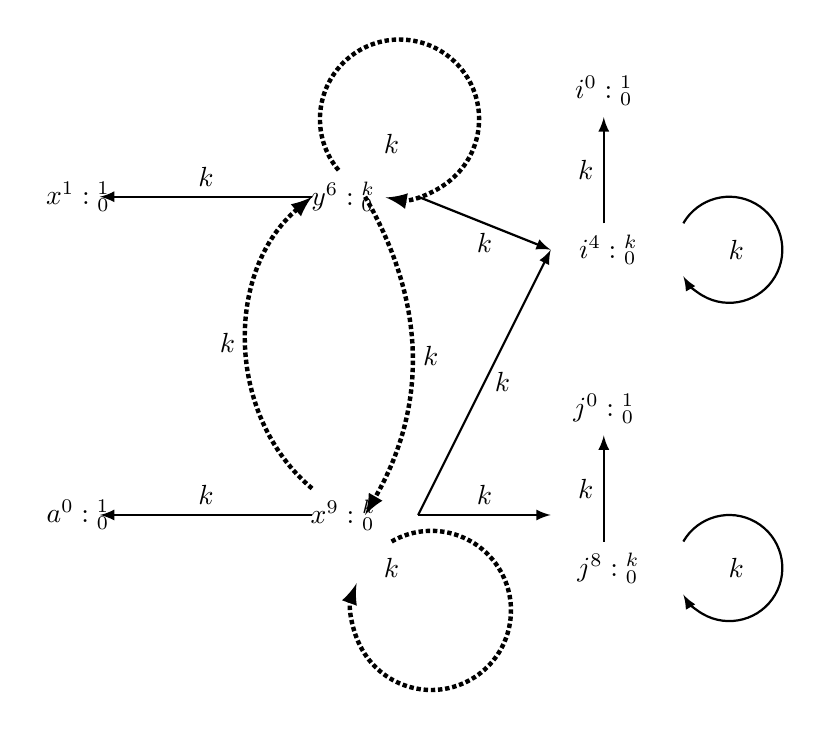
\begin{tikzpicture}[scale=\textwidth/18cm,samples=200]
      % Variables Initialization
      \draw[] (-5, 1) circle (0pt) node{{ $a^0: {}^1_{0}$}};
      \draw[] (-5, 7) circle (0pt) node{{ $x^1: {}^{1}_{0}$}};
      % Variables Inside the Loop
      \draw[] (0, 7) circle (0pt) node{{ $y^6: {}^{k}_{0}$}};
      \draw[] (0, 1) circle (0pt) node{{ $x^9: {}^{k}_{0}$}};
      % Counter Variables
      \draw[] (5, 9) circle (0pt) node {{$i^0: {}^{1}_{0}$}};
      \draw[] (5, 6) circle (0pt) node {{ $i^4: {}^{k}_{0}$}};
      \draw[] (5, 3) circle (0pt) node {{$j^0: {}^{1}_{0}$}};
      \draw[] (5, 0) circle (0pt) node {{ $j^8: {}^{k}_{0}$}};
      % Value Dependency Edges:
      \draw[ ultra thick, -latex, densely dotted,] (0, 7.5) arc (220:-100:1.5);
      \draw[] (1, 8) node [] {\highlight{$k$}};
      \draw[ thick, -latex] (5, 6.5)  -- node[left]{\highlight{{$k$}}}(5, 8.5) ;
      \draw[ thick, -latex] (5, 0.5)  -- node[left]{\highlight{{$k$}}}(5, 2.5) ;
      \draw[ ultra thick, -latex, densely dotted,] (1., 0.5) arc (120:-200:1.5);
      \draw[] (1, 0) node [] {\highlight{$k$}};
      % Value Dependency Edges on Initial Values:
      \draw[ thick, -latex,] (-0.5, 1)  -- node[above]{\highlight{{$k$}}}(-4.5, 1) ;
      \draw[ thick, -latex,] (-0.5, 7)  -- node[above]{\highlight{{$k$}}}(-4.5, 7) ;
      %
      \draw[ ultra thick, -latex, densely dotted,] (-0.5, 1.5)  to  [out=-220,in=220]  
      node[left]{\highlight{{$k$}}}(-0.5, 7);
      \draw[ ultra thick, -latex, densely dotted,]  (0.5, 7) to  [out=-60,in=60] 
      node[right]{\highlight{{$k$}}}(0.5, 1) ;
      % Control Dependency
      \draw[ thick, -latex, ] (6.5, 6.5) arc (150:-150:1);
      \draw[] (7.5, 6) node [] {\highlight{$k$}};
      \draw[ thick, -latex, ] (6.5, 0.5) arc (150:-150:1);
      \draw[] (7.5, 0) node [] {\highlight{$k$}};
      \draw[ thick,-latex] (1.5, 7)  -- node[below]{\highlight{{$k$}}}(4, 6) ;
      \draw[ thick,-latex] (1.5, 1)  -- node[right]{\highlight{{$k$}}}(4, 6) ;
      \draw[ thick,-latex] (1.5, 1)  -- node[above]{\highlight{{$k$}}}(4, 1) ;
   \end{tikzpicture}
   \caption{}
      \end{centering}
      \end{subfigure}
    }
     \caption{(a) Nested While Loop Example, (b) Execution-Based Dependency Graph, (c) The Static Program-Based Dependency graph.}
    \label{fig:alg_adaptsearch_nestedwhile}
    \vspace{-0.5cm}
    \end{figure}
  \end{example}

\subsection{Proposed Methodology}
\label{subsubsec:furthers-cost-methodology}
Following the same system structure as $\THESYSTEM$,
by modifying the restriction on finite walk, compute different resource cost for program.

